% --------------------------------------------------------------
% This is all preamble stuff that you don't have to worry about.
% Head down to where it says "Start here"
% --------------------------------------------------------------

\documentclass[10pt]{beamer}

% \usepackage[margin=1in]{geometry}
\usepackage{amsmath,amsthm,amssymb}
\usepackage{enumitem}
\usepackage{tikz}
\usepackage{wrapfig}
\usepackage{cjhebrew}
% \usepackage[shortlabels]{enumerate}

\usepackage[utf8]{inputenc}
\usepackage[english]{babel}

\usetikzlibrary{calc}
\usetikzlibrary{arrows.meta}
\usetikzlibrary{arrows}

\newcommand{\NN}{\mathbb{N}}
\newcommand{\ZZ}{\mathbb{Z}}
\newcommand{\QQ}{\mathbb{Q}}
\newcommand{\RR}{\mathbb{R}}
\newcommand{\CC}{\mathbb{C}}

\newcommand{\CVect}{\CC\operatorname{-Vect}}
\newcommand{\card}{\operatorname{card}}
\newcommand{\diam}{\operatorname{diam}}
\newcommand{\id}{\operatorname{id}}
\newcommand{\interior}{\operatorname{int}}
\newcommand{\lcm}{\operatorname{lcm}}
\newcommand{\Lip}{\operatorname{Lip}}
\newcommand{\norm}[1]{\left\lVert#1\right\rVert}

\newcommand{\Spec}{\operatorname{Spec}}

\renewcommand{\Re}{\operatorname{Re}}
\renewcommand{\Im}{\operatorname{Im}}

\newtheorem{conjecture}{Conjecture}
\newtheorem{question}{Question}
\newtheorem{assumption}{Assumption}

\usepackage[backend=bibtex,style=alphabetic,maxcitenames=50,maxnames=50]{biblatex}
\addbibresource{supermartingales.bib}
\renewbibmacro{in:}{}
\DeclareFieldFormat{pages}{#1}

\newcommand{\attn}[1]{\textbf{\textcolor{blue}{#1}}}

\usetheme{AnnArbor}
\usecolortheme{dove}

\begin{document}
\title{The House Always Wins}
\author{Aidan Backus}
% --------------------------------------------------------------
%                         Start here
% --------------------------------------------------------------
\begin{frame}
    \titlepage
\end{frame}

\begin{frame}{The House Always Wins}
\begin{theorem}[Doob's optional stopping theorem, 1953]
No matter which strategy a gambler uses, her expected return is always nonpositive.
\end{theorem}

Before we can prove it, we need to make this precise: what strategies are allowed? What rules is the casino playing by? What assumptions on gambler's initial capital?

\begin{center}
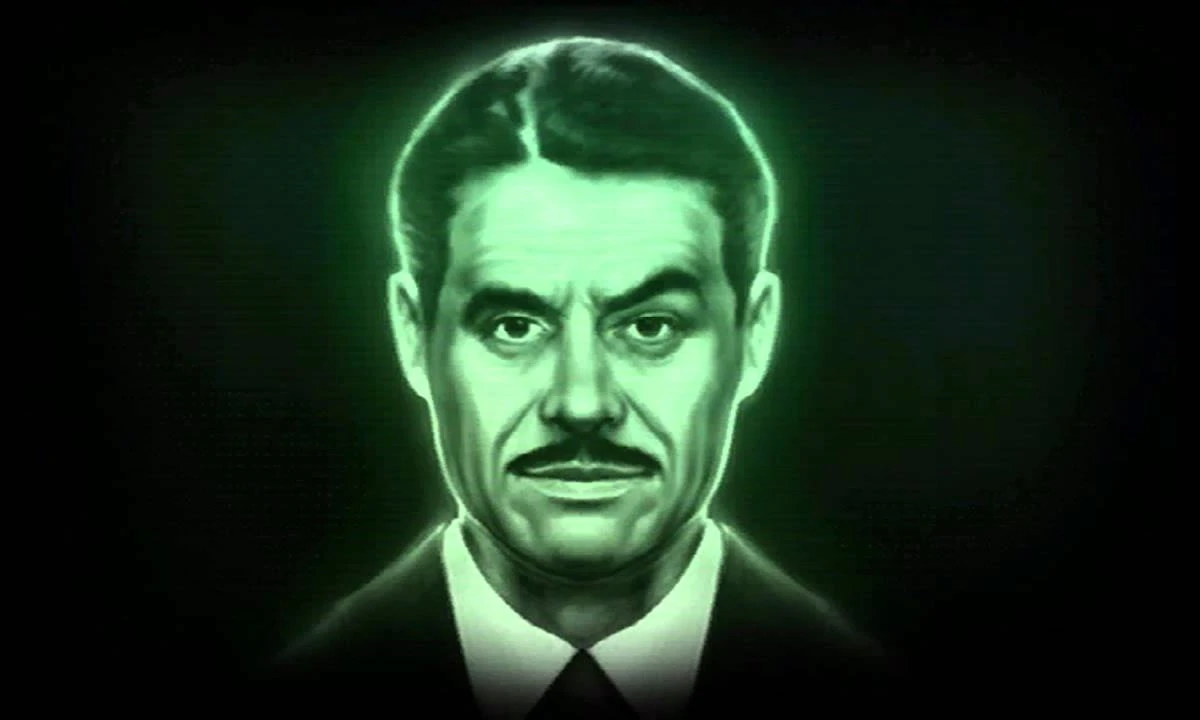
\includegraphics[scale=0.15]{Mr._House}
\end{center}
\end{frame}

\begin{frame}{A little measure theory}
We need a way to model how much information our gambler Alice has...

Given events $A, B$ will use $A \cap B$ to mean $A$ AND $B$, $A \cup B$ to mean $A$ OR $B$, $A^c$ to mean NOT $A$.
We will use $\Omega$ to mean the event which is always TRUE.

\begin{definition}
A \emph{$\sigma$-algebra} is a set $\mathcal F$ of events such that:
\begin{itemize}
\item $\Omega \in \mathcal F$.
\item If $A_1, A_2, \dots \in \mathcal F$ then $A_1 \cap A_2 \cap \cdots \in \mathcal F$.
\item If $A \in \mathcal F$ then $A^c \in \mathcal F$.
\end{itemize}
\end{definition}

The set of events whose truth value we know is a $\sigma$-algebra: if we know whether $A,B$ are true, then we know whether $A^c$ is true, whether $A \cap B$ is true, etc., and of course we always know that $\Omega$ is true. So $\sigma$-algebras hold information: the bigger the $\sigma$-algebra, the more information we have.
\end{frame}

\begin{frame}{A little measure theory}
Recall conditional expectation: given a random variable $X$ and event $A$, the conditional expectation $E(X|A)$ is the mean of $X$ over all outcomes $\omega$ such that $\omega \in A$ -- it's the expected value of $X$ if Alice knows that $A$ is true.

\begin{definition}
Let $X$ be a random variable and $\mathcal F$ a $\sigma$-algebra.
The \emph{conditional expectation} $E(X|\mathcal F)$ is the unique\footnote{If $X \in L^1$, this is well-defined by the Radon-Nikod\'ym theorem.} random variable such that:
\begin{itemize}
\item If we know the truth value of every event in $\mathcal F$, we can determine $E(X|\mathcal F)$.
\item For every $A \in \mathcal F$,
$$E(E(X|\mathcal F)|A) = E(X|A).$$
\end{itemize}
\end{definition}

Intuitively, if $\mathcal F$ is the $\sigma$-algebra of all information that Alice has, $E(X|\mathcal F)$ is her best guess at what $X$ is.
\end{frame}

\begin{frame}{A little measure theory}
\begin{definition}
A \emph{history} $\mathcal F$ consists of $\sigma$-algebras $\mathcal F_t$ for all times $0 \leq t \leq s$, $\mathcal F_t \subseteq \mathcal F_s$.
\end{definition}

The history records how much information Alice has at each time.
At time $t$ she knows the truth value of all the events in $\mathcal F_t$.
As time goes on, she learns more stuff and so she has more information.
\end{frame}

\begin{frame}{Supermartingales}
Let $X_t$ be the Alice's capital at time $t$ and let $\mathcal F_t$ be the $\sigma$-algebra which records the values of $X_1, \dots, X_t$.
Then $\mathcal F$ is a history.

At each time $t$, Alice bets some quantity on a game $G_t$.

\begin{assumption}[no time travel]
Alice is allowed to decide how much to bet on $G_t$ using information from $\mathcal F_t$, but cannot use any information from $\mathcal F_s$ for any $s > t$.
\end{assumption}

Let $Y_t$ be Alice's net winnings from $G_t$. Then $X_{t + 1} = X_t + Y_t$, and if Alice bets nothing on $G_t$, then $Y_t = 0$.

\begin{assumption}[individual games are rigged]
The casino has rigged each game $G_t$ so that, regardless what Alice bets on $G_t$, Alice's net winnings from $G_t$ are nonpositive, thus
$$-\infty < E(Y_t|\mathcal F_t) \leq 0.$$
\end{assumption}
\end{frame}

\begin{frame}{Supermartingales}
\begin{definition}
A \emph{supermartingale} consists of random variables $X_t$ for every time $t \geq 0$, such that if $t \geq s$, then
$$E(X_t|\mathcal F_s) \leq X_s,$$
where $\mathcal F_s$ is the smallest history such that for every $r \leq s$, $\mathcal F_s$ knows the value of $X_s$.
\end{definition}

In other words, a supermartingale is a quantity $X$ that is allowed to change over time, but if we know the value $X_s$ of $X$ at time $s$, and $t \geq s$, then we expect $X_t$ to be at most its current value $X_s$.

Let $X_t$ be Alice's capital at time $t$ and $Y_t$ her net winnings from the game $G_t$, which is determined by $\mathcal F_t$ since there is \attn{no time travel}. Then
$$E(X_{t + 1}|\mathcal F_t) = X_t + E(Y_t|\mathcal F_t) \leq X_t$$
since \attn{individual games are rigged}. So $X$ is a supermartingale.
\end{frame}

\begin{frame}{Stopping times}
In the Ancien Régime, the ``martingale" was a popular betting strategy: Alice doubles her bet every game, so that, when she eventually wins, she wins back everything she's bet so far and then some.
So, once Alice finally wins a game, she'll stop playing and come out ahead, even though her capital is a supermartingale.
This apparent contradiction is called the \emph{St. Petersberg paradox}.

Doob solved the St. Petersberg paradox under the following assumption:

\begin{assumption}[finite capital resources]
Alice's initial capital $X_0$ and credit limit $M$ are both finite ($\max(X_0, M) < \infty$), and she must stop playing at time $t$ if $X_t \leq -M$.
\end{assumption}
\end{frame}

\begin{frame}{Stopping times}
\begin{definition}
Let $\mathcal F$ be a history.
A \emph{stopping time} for $\mathcal F$ is a random time $\tau$ such that for every deterministic time $t$, the event $\{\tau \leq t\} \in \mathcal F_t$.
\end{definition}
If $\tau \leq t$, that means we must have stopped at time $t$.

Let $\tau$ be the time that Alice stops gambling.
Since Alice has \attn{finite capital resources}, if $X_t \leq -M$, then $\tau \leq t$.

Since there is \attn{no time travel}, if $\tau \leq t$ (thus $\tau = 1$, $\tau = 2$, ..., or $\tau = t$) then Alice must have made the decision to stop gambling based on her performance in games $G_1, \dots, G_t$, but not on her performance in games $G_s$ where $s > t$.
Thus Alice will be able to tell whether $\tau \leq t$ based on just the information in $\mathcal F_t$, so $\{\tau \leq t\} \in \mathcal F_t$.
Therefore $\tau$ is a stopping time.
\end{frame}

\begin{frame}{Stopping times}
\begin{definition}
Let $X$ be a supermartingale with history $\mathcal F$, and let $\tau$ be a stopping time for $\mathcal F$.
The \emph{stopped supermartingale} $X^\tau$ consists of the random variables $X^\tau_t = X_{\min(\tau, t)}$ for every time $t \geq 0$.
\end{definition}

Our running assumptions say that Alice's capital, if she were to keep playing forever, would be a supermartingale $X$.
However, she can stop playing at a stopping time $\tau$ (and in fact MUST stop, if her debt exceeds her credit limit).
So, in reality, her capital is better modelled as the stopped supermartingale $X^\tau$.
But that's not a problem, because:

\begin{theorem}[Doob's optional stopping theorem, 1953]
Every stopped supermartingale is a supermartingale.
\end{theorem}
\end{frame}

\begin{frame}{The House Really Does Always Win}
We want to know the expected value of $X_\tau$, the amount of capital Alice has when she stops playing. But
$$X_\tau = \lim_{t \to \infty} X_{\min(\tau, t)} = \lim_{t \to \infty} X_t^\tau.$$
(One needs to check that this limit exists -- this follows from the martingale convergence theorem, \attn{finite capital resources}, and \attn{individual games are rigged}.)

Then
$$EX_\tau = E\left(\lim_{t \to \infty} X_t^\tau\right) \leq \lim_{t \to \infty} EX_t^\tau$$
by Fatou's lemma and \attn{finite capital resources}.

But $X^\tau$ is a supermartingale by Doob's optional stopping theorem, so
$$EX_t^\tau \leq EX_0^\tau = X_0.$$
Therefore $EX_\tau \leq X_0$. So, the house really does always win.
\end{frame}

\begin{frame}{Brownian motion}
Recall that a supermartingale $X$ satisfies $E(X_t|\mathcal F_s) \leq X_s$.

\begin{definition}
A \emph{martingale} consists of random variables $X_t$, such that if $\mathcal F$ is the history of $X$, then
$$E(X_t|\mathcal F_s) = X_s.$$
\end{definition}

A martingale models Alice's capital in a casino where every game has expected return zero (as opposed to nonpositive expected return).
\end{frame}

\begin{frame}{Brownian motion}
\begin{definition}
The $d$-dimensional \emph{Brownian motion} $W$ is the\footnote{well-defined as a probability measure, as one can show using Fourier series} random continuous function $W: [0, \infty) \to \RR^d$, such that:
\begin{itemize}
\item $W_0 = 0$.
\item \emph{Independent increments}: Let $0 < s < t$ and $\mathcal F$ be the history of $W$. Then $W_t - W_s$ is a $N(0, t - s)$ random variable independent of $\mathcal F_s$.
\end{itemize}
\end{definition}
\attn{Independent increments} implies that Brownian motion is a martingale:
$$E(W_t|\mathcal F_s) = W_s - E(W_t - W_s|\mathcal F_s) = W_s - E(W_t - W_s) = W_s.$$
It means that at every time, a particle traveling along Brownian motion forgets its current velocity and goes whichever which way it feels like.
The assumption that the distribution is normal is justified by the central limit theorem.

See \attn{\href{https://upload.wikimedia.org/wikipedia/commons/5/51/Brownianmotion5particles150frame.gif}{animation}}, the blue trajectories are Brownian motion.

\end{frame}

\begin{frame}{Stochastic calculus}
\begin{theorem}
Most\footnote{in the sense of the Baire category theorem} continuous functions $[0, \infty) \to \RR$ are not differentiable ANYWHERE.
\end{theorem}

The first example of such a function was Weierstrass' Monster $\sum_{n=0}^\infty a^n \cos(7^n \pi x)$
where $a < 1$ is large enough. But Brownian motion is also not differentiable anywhere.
Essentially this is because at any time $t$, Brownian motion doesn't remember where it was going, by \attn{independent increments}.

\begin{center}
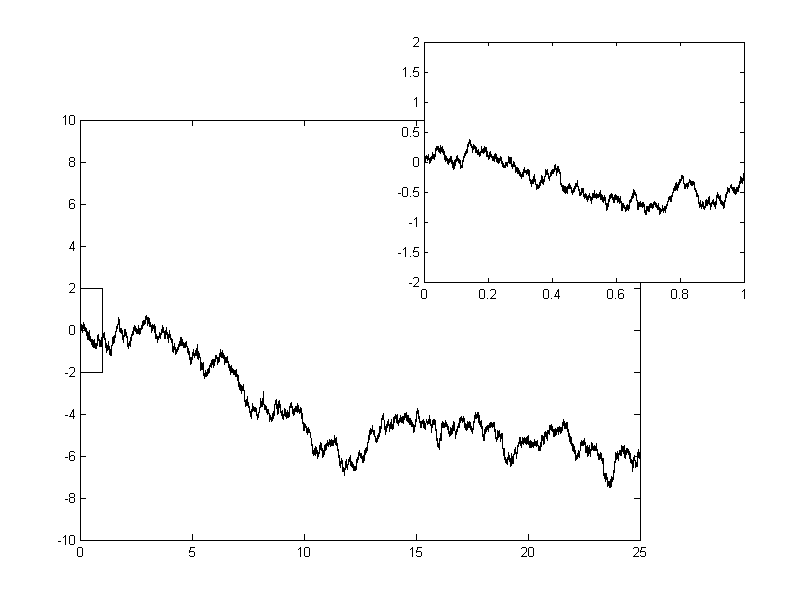
\includegraphics[scale=0.25]{Wiener_process_zoom}
\end{center}
\end{frame}

\begin{frame}{Stochastic calculus}
Since Brownian motion isn't differentiable, we need to change up the chain rule...
\begin{theorem}[It\^o's chain rule]
Let $\mathcal F$ be the history of the Brownian motion $W$.
Let $f$ be a deterministic smooth function and $\mu,\sigma$ random continuous functions such that $\mu_t,\sigma_t$ are determined by information in $\mathcal F_{t - \epsilon}$. Let $X$ be a random function which solves the differential equation
$$dX_t = \mu_t ~dt + \sigma_t ~dW_t.$$
Then
$$d(f(X_t)) = f'(X_t)~dX_t + \sigma^2 \frac{f''(X_t)}{2} ~dt.$$
\end{theorem}

Applications of Brownian motion using calculus include the fundamental theorem of algebra, Atiyah-Singer index theory (whose consequences include the Gauss-Bonnet and Riemann-Roch theorems), and the fact that Avogadro's number is $6 \cdot 10^{23} + O(10^{21})$.
\end{frame}

%\begin{frame}{Calculus and Brownian motion}
%\begin{theorem}
%Let $\rho$ be the number density of particles, all of which move according to independent Brownian motions.
%Then there is a ``diffusion constant" $\alpha > 0$ such that $\rho$ solves the heat equation
%$$\partial_t \rho = \alpha \Delta \rho$$
%\end{theorem}
%This theorem was essential to the development of the kinetic molecular theory.
%It can also be used to prove the famous Atiyah-Singer index theorem, whose consequences include the Gauss-Bonnet and Riemann-Roch theorems.
%\end{frame}

%\begin{frame}{Kinetic molecular theory}
%Some history:
%\begin{itemize}
%\item 60 BCE: Lucretius observes that dust particles in water move according to Brownian motion.
%\item 1827 CE: Robert Brown documents \emph{C. pulchella} pollen particles in water moving according to Brownian motion.
%\item 1905 CE: Albert Einstein notices that Brownian motion can be described by collisions with water molecules, uses this as strong evidence for %kinetic molecular theory.
%\item 1926 CE: Norbert Wiener defines Brownian motion rigorously.
%\item 1944 CE: Kiyoshi It\^o defines the integral $\int_0^t Z_s ~dW_s$ of a random continuous function $Z$ against Brownian motion, and proves his %chain rule.
%\end{itemize}
%\end{frame}

%\begin{frame}{Kinetic molecular theory}
%Let $\rho$ be the number density of \emph{C. pulchella} pollen particles.
%Then we have
%$$\frac{\partial \rho}{\partial t} = \alpha \Delta \rho.$$
%Einstein showed that
%$$\alpha = \frac{RT}{6\pi\eta rN_A}$$
%where $R$ is the ideal gas constant, $T$ is the temperature, $\nu$ is the viscosity of water, $r$ is the pollen particle radius, and $N_A$ is %Avogadro's number.
%By experimentally measuring $\alpha$, one can compute
%$$N_A = 6 \cdot 10^{23} + O(10^{21}) \frac{\text{molecules}}{\text{mole}},$$
%where a mole is the number of molecules in $18.015$ grams of water.
%\end{frame}

\begin{frame}{Black-Scholes theory}
The value of a stock undergoes a lot of random fluctuations:

\begin{center}
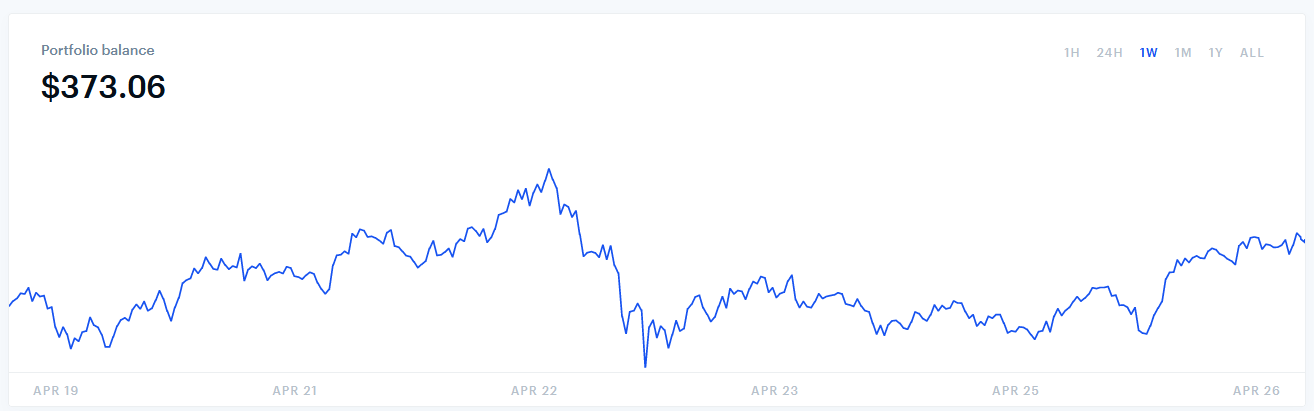
\includegraphics[scale=0.3]{HODL}
\end{center}

So we should expect Brownian motion to enter into any realistic model of the stock market.
\end{frame}

\begin{frame}{Black-Scholes theory}
Let $S$ be the price of a stock, say for GameStop.
\begin{assumption}[stochastic continuous compounding]
The price $S$ solves the differential equation
$$\frac{dS}{S} = \mu ~dt + \sigma ~dW.$$
where $\mu,\sigma$ are constants. Here $\mu$ is the interest rate and $\sigma$ is the uncertainty.
\end{assumption}
By It\^o's chain rule, we have
$$S_t = S_0 \exp\left(\mu t - \frac{\sigma^2}{2} t + \sigma W_t\right).$$
So \attn{stochastic continuous compounding} is a modification of the classical ``continuously compounding" model $S_t = S_0 e^{\mu t}$ you learned about in high school Algebra II to account for redditors randomly buying up GameStop stock.
\end{frame}

\begin{frame}{Black-Scholes theory}
Suppose that Bob owns stock in GameStop. At time $0$, Bob buys a \emph{European put} from Eve for some price $V$. This is a contract which fixes a \emph{strike price} $P$ and expiry time $T$ and allows him to sell his GameStop stock to Eve at any time in $[0, T]$ he wants at price $P$, even if $S$ is much smaller than $P$.
Thus Bob is betting that $S$ will dip while Eve is betting that it will stay high.

Black-Scholes theory allows us to compute $V$ -- how much should Eve charge Bob for a European put?

We are given that $V$ is a function of $S$ and time. By \attn{stochastic continuous compounding} and It\^o's chain rule,
$$dV = \left(\mu S \frac{\partial V}{\partial S} + \frac{\partial V}{\partial t} + S^2 \frac{\sigma^2}{2} \frac{\partial^2 V}{\partial S^2}\right) ~dt + \sigma S \frac{\partial V}{\partial S} ~dW.$$
\end{frame}

\begin{frame}{Black-Scholes theory}
Now consider an asset $\mathcal P$ whose value is
$$\Pi = \frac{\partial V}{\partial S}S - V.$$
Plugging in $dV$ and $dS$, the Brownian motion terms all vanish:
$$\frac{\partial \Pi}{\partial t} = -\frac{\partial V}{\partial t} - S^2\frac{\sigma^2}{2} \frac{\partial^2 V}{\partial S^2}.$$
Thus $\mathcal P$ has no uncertainty; it is a \emph{risk-free asset}.

\begin{assumption}[no arbitrage]
There is a UNIQUE interest rate for risk-free assets.
\end{assumption}

\attn{No arbitrage} makes sense because if it was not true, and $\mathcal Q_1,\mathcal Q_2$ were risk-free assets with interest rates $r_1,r_2$, and $r_1 > r_2$, every rational agent would sell $\mathcal Q_2$ to buy $\mathcal Q_1$, driving down $r_1$ and driving up $r_2$. One can think of ``risk-free assets" as a model for the US dollar.
\end{frame}

\begin{frame}{Black-Scholes theory}
By \attn{no arbitrage}, there is a constant $r > 0$, which only depends on the market and not the stocks involved, such that
$$\frac{\partial \Pi}{\partial t} = r\Pi.$$
But we already had a PDE for $\Pi$, so plugging everything in we deduce:
\begin{theorem}[Black-Scholes 1973]
Let $r$ be the risk-free interest rate in a market with \attn{no arbitrage}.
If a stock $\mathcal P$ with value $S$ and uncertainty $\sigma$ satisfies \attn{stochastic continuous compounding}, then the value $V$ of a European put for $\mathcal P$ which expires at time $T$ with strike price $P$ is the unique solution of the terminal-value problem
\begin{align*}
r\left(\frac{\partial V}{\partial S}S - V\right) + \frac{\partial V}{\partial t} + S^2\frac{\sigma^2}{2} \frac{\partial^2 V}{\partial S^2} &= 0\\
V_T &= \max(S_T - P, 0).
\end{align*}
\end{theorem}
\end{frame}



\end{document}
